\chapter{Aplicaciones Proyectivas}
\label{C4}
En este capítulo vamos a tratar de extrapolar uno de los conceptos más centrales del álgebra lineal al contexto proyectivo. Tratamos de estudiar las aplicaciones entre espacios proyectivos cuyo comportamiento consideramos ``bueno''.

En el mundo lineal, estas aplicaciones eran los llamados homomorfismos entre espacios vectoriales o símplemente aplicaciones lineales. Aquí, en el mundo de los rayos, las llamaremos \ti{aplicaciones proyectivas}.
\section{Definición}
\label{C4_definicion}
Sean dos espacios proyectivos $X$ e $Y$ asociados a sendos espacios vectoriales, $\widehat{X}$ e $\widehat{Y}$ respectivamente.

Nuestro objetivo es definir una aplicación proyectiva entre dos espacios proyectivos a partir de una aplicación lineal entre sus respectivos espacios lineales de forma natural. Intentémoslo y veamos qué dificultades se nos presentan.

Sea $\widehat{h}:\widehat{X}\to\widehat{Y}$ una aplicación lineal arbitraria. Lo deseable sería definir la aplicación proyectiva asociada a $\widehat{h}$ como aquella que, a cada rayo le asigna el rayo engendrado por la imagen de uno de sus representantes. Visto formalmente, si $x=\class{u}$:
\[\begin{array}{c}
X\stackrel{h}{\to}Y\\
x\mapsto\class{\widehat{h}(u)}
\end{array}\]
Este intento de definición tan intuitivo e inocente presenta dos problemas. El primero de ellos es que si $\widehat{h}(u)=0$ entonces el rayo $\class{\widehat{h}(u)}$ no está definido.

Esto lo arreglamos de una forma natural, restringiendo el dominio de $\widehat{h}$ a los vectores de $\widehat{X}$ que no se anulan mediante $\widehat{h}$. Es decir, ahora $\widehat{h}$ queda definida en $\widehat{X}\setminus \ker\left(\widehat{h}\right)$.

Trasladando esta restricción al contexto proyectivo obtenemos este segundo intento de definición de aplicación proyectiva asociada a cierta aplicación lineal:
\[\begin{array}{c}
X\setminus\proy\left(\ker\left(\widehat{h}\right)\right)\stackrel{h}{\to}Y\\
x\mapsto\class{\widehat{h}(u)}
\end{array}\]
Antes de hacer algunas aclaraciones adicionales acerca de este primer problema que se nos ha presentado, demos una pequeña definición (por comodidad tipográfica).
\begin{defi}[Centro]
	\label{C4_def_centro}
	Se denomina \ti{centro} de una aplicación $h$, dada la aplicación lineal asociada $\widehat{h}$ entre dos espacios lineales $\widehat{X}$ e $\widehat{Y}$, a la variedad proyectiva:
	\[\mc{Z}:\equals{not.}\proy\left(\ker\left(\widehat{h}\right)\right)\]
\end{defi}
Tras este breve inciso sobre la notación, veamos que, en efecto, hemos resuelto el problema que se nos planteaba, es decir, hemos eliminado del dominio todos los rayos que no tenían imagen definida. Si hubiera algún rayo con imagen no definida, alguno de sus representantes debería pertenecer al núcleo de $\widehat{h}$ (y por tanto todos). Pero esto no es posible ya que el rayo engendrado por este representante estaría en el centro de $h$.

El segundo problema que planteaba nuestra definición era saber si está bien definida. En efecto, siempre que definamos una aplicación y los elementos de nuestro conjunto de salida no tengan una representación única, debemos comprobar que la imagen de la función es independiente del representante escogido. En este caso es un juego de niños:

Sean $\class{u'}=x=\class{u}$. Es evidente que $u' = \lambda u$ para cierto $\lambda$ no nulo. Entonces:
\[\class{\widehat{h}(u')}=\class{\widehat{h}(\lambda u)}=\class{\lambda\widehat{h}(u)}=\class{\widehat{h}(u)}\]

Para terminar la sección advertimos de que en algunos textos, a la hora de representar una aplicación proyectiva omiten (abusando de notación) especificar que al espacio de partida se le extrae el centro $\mc{Z}$. 
\section{Propiedades Elementales}
En esta sección estudiaremos diversas propiedades básicas de las aplicaciones proyectivas.

Comencemos viendo cuál es la relación entre las aplicaciones proyectivas inyectivas (y respectivamente sobreyectvas) y sus aplicaciones lineales asociadas.
\begin{lem}[Inyectividad y Sobreyectividad]
	\label{C4_lem_inyectividadSobreyectividad}
	Sea $h$ una aplicación proyectiva. Se cumple:
	\begin{enumerate}
		\item $h$ es inyectiva si y solo si lo es $\widehat{h}$.
		\item $h$ es sobreyectiva si y solo si lo es $\widehat{h}$.
	\end{enumerate}
\end{lem}
\begin{proof}
	\begin{enumerate}
		\item Suponiendo que $h$ es inyectiva, si $\widehat{h}$ no lo fuera, entonces tendría un núcleo no trivial, es decir, existiría cierto $u\not=0$ tal que $\widehat{h}(u)=0$. A su vez, como $\widehat{h}$ no puede ser la aplicación idénticamente nula, existirá un $v\not=0$ de manera que $\widehat{h}(v)\not=0$. Es un ejercicio trivial (que se deja al lector) la comprobación de que los vectores $v$ y $w=u+v$ son linealmente independientes. Esto quiere decir que los puntos proyectivos $x=\class{v}$ e $y=\class{w}$ son distintos. Sin embargo, al tomar sus imágenes por $h$ obtenemos:
		\[h(y)=\class{\widehat{h}(w)}=\class{\widehat{h}(u+v)}=\class{\widehat{h}(u)+\widehat{h}(v)}=\class{\widehat{h}(v)}=h(x)\]
		Lo cual contradice nuestra hipótesis. Recíprocamente, si $\widehat{h}$ es inyectiva, usando la definción de aplicación proyectiva y la linealidad e inyectividad de $\widehat{h}$ tenemos que:
		\begin{multline}
			h(x)=h(y)\sii h(\class{u})=h(\class{v})\sii\class{\widehat{h}(u)}=\class{\widehat{h}(v)}\sii\\\sii\widehat{h}(u)=\lambda \widehat{h}(v)\sii\widehat{h}(u)=\widehat{h}(\lambda v)\sii u = \lambda v\sii\class{u}=\class{v}\sii x=y
		\end{multline}
		\item Suponiendo que $\widehat{h}$ es sobreyectiva, dado un $y\in Y$, veamos que existe un $x\in X\setminus\mc{Z}$ tal que $h(x)=y$. En efecto, $y=\class{v}$, como $\widehat{h}$ es sobreyectiva, existe un $u\in \widehat{X}$ tal que $\widehat{h}(u)=v$, luego, tomando clases:
		\[h(x)=\class{\widehat{h}(u)}=\class{v}=y\]
		Recíprocamente, si $h$ es sobreyectiva, dado $v\in\widehat{Y}$ es claro que existe un $x\in X\setminus\mc{Z}$ tal que: 
		\[h(x)=\class{\widehat{h}(u)}=\class{v}\]
		Luego $v=\widehat{h}(\lambda u)$, lo que prueba la sobreyectividad de $\widehat{h}$.
	\end{enumerate}
\end{proof}
\begin{cor}[Biyectividad]\label{C4:cor_biyectividad}
	Una aplicación proyectiva es biyectiva si y solo si su aplicación lineal asociada es un isomorfismo.
\end{cor}

Veamos con un ejemplo que ya, con lo poco que sabemos podemos demostrar cosillas bastante interesantes:
\begin{exa}[Aplicaciones No Inyectivas Constantes]
	Veamos que las aplicaciones proyectivas no inyectivas que parten de un subespacio proyectivo de dimensión $1$ son constantes.
	
	Para ello usamos el lema \ref{C4_lem_inyectividadSobreyectividad}. Si una aplicación cumpliera las características de nuestra hipótesis, su aplicación lineal correspondiente partiría de un espacio vectorial de dimensión $2$ y tampoco sería inyectiva, siendo su núcleo un subespacio de dimensión $1$ y su imagen otro subespacio de dimensión $1$. Al proyectivizar nos que nuestra aplicación parte de un espacio proyectivo de dimensión $1$ (extrayendo el punto asociado al núcleo) y llega a un espacio proyectivo conformado por un único punto (el proyectivizado de la imagen de su aplicación lineal).
\end{exa}
Veamos ahora que, tanto la imagen como la imagen inversa de una variedad por una aplicación proyectiva es otra variedad.
\begin{lem}[Preservación de Variedades]
	\label{C4_lem_preservaVariedades}
	Sea $h:X\setminus\mc{Z}$ una aplicación proyectiva se cumple que:
	\begin{enumerate}
		\item Dada una variedad $W\subset X$, entonces $h(W\setminus\mc{Z})$ es una variedad de $Y$. Además: \[\pi^{-1}\left(h(W\setminus \mc{Z})\right)=\widehat{h}(\widehat{W})\]
		\item Dada una variedad $W'\subset Y$, entonces $h^{-1}(W')\cup\mc{Z}$ es una variedad de $X$. Además: \[\pi^{-1}\left(h^{-1}(W')\cup\mc{Z}\right)=\widehat{h^{-1}}(\widehat{W'})\]
	\end{enumerate}
\end{lem}
\begin{proof}
	Probaremos únicamente el segundo apartado (el otro se demuestra de forma análoga). Probemos en primer lugar el ``además'', de donde deduciremos automáticamente el resultado.
	
	Sea $w\in \widehat{h^{-1}}(\widehat{W'})$. Esto es equivalente a decir que $\widehat{h}(w)\in\widehat{W'}$. En caso de que $\widehat{h}(w)=0$ tendríamos que $\class{w}\in\mc{Z}$. En caso contrario tenemos:
	\[\class{\widehat{h}(w)}=h(\class{w})\in W'\sii\class{w}\in h^{-1}(W')\]
	Saltando al espacio lineal, combinando ambos casos, tenemos que:
	\[w\in\pi^{-1}\left(h^{-1}(W')\cup\mc{Z}\right)\]
	Como todos los pasos que hemos hecho son equivalencias, también tenemos el otro contenido.
	
	Como $\widehat{h^{-1}}(\widehat{W'})$ es un subespacio vectorial, $\pi^{-1}\left(h^{-1}(W')\cup\mc{Z}\right)$ también lo es, y por ende, al proyectivizar obtendremos una variedad proyectiva, que es precisamente $h^{-1}(W')\cup\mc{Z}$.
\end{proof}

Pasemos a comprobar cómo se comportan las aplicaciones proyectivas respecto de la composición.
\begin{lem}[Composición de Aplicaciones Proyectivas]
	\label{C4_lem_composicionProyectivas}
	La composición de dos aplicaciones proyectivas ($f$ y $g$) es una aplicación proyectiva, siempre y cuando la composición de sus respectivas aplicaciones lineales asociadas no sea idénticamente nula ($\widehat{f}\circ \widehat{g}\not=0$).
	
	Además, $\widehat{f\circ g}=\widehat{f}\circ\widehat{g}$.
\end{lem}
\begin{proof}
	Demostrando el ``además'' el resultado se sigue:
	\[\begin{array}{c}X_1\setminus\mc{Z}_1 \stackrel{g}{\to} X_2\setminus\mc{Z}_2 \stackrel{f}{\to} X_3\\
	\class{u} \mapsto g(\class{u})=\class{\widehat{g}(u)} \mapsto (f\circ g)(\class{u})=f(\class{\widehat{g}(u)})=\class{\widehat{f}(\widehat{g}(u))}=\class{(\widehat{f}\circ\widehat{g})(u)}
	\end{array}\]
	Además, nótese que $\widehat{\mc{Z}_1}\subset\ker(\widehat{f}\circ\widehat{g})$ y por ende $\widehat{g^{-1}}(\widehat{\mc{Z}_2})=\ker(\widehat{f}\circ\widehat{g})$. Esto quiere decir:
	\[\mc{Z}=\proy(\widehat{g^{-1}}(\widehat{\mc{Z}_2}))\]
	Por ende $\widehat{f}\circ \widehat{g}=0\sii \widehat{g}(\widehat{X_1})\subset\widehat{\mc{Z}_2}$.
\end{proof}

Un resultado deseable, aunque para nada inmediato, es el de que podamos clasificar a las aplicaciones lineales que inducen cierta aplicación proyectiva por ser múltiplos entre si. Veamoslo:
\begin{theo}[Lema de la Correspondencia]
	\label{C4_teo_lemaCorrespondencia}
	Dos aplicaciones lineales no nulas producen la misma aplicación proyectiva si y solo si son múltiplos la una de la otra.
\end{theo}
\begin{proof}
	\begin{itemize}
		\item[$\bra$] Sean dos aplicaciones lineales $\widehat{g},\widehat{h}:E\to E'$ tales que inducen la misma aplicación proyectiva. Esto es:
		\[\begin{array}{c}
		\proy(E)\setminus\mc{Z}\stackrel{\varphi}{\to}\proy(E')\\
		x=\class{u}\mapsto\varphi(x)=\class{\widehat{g}(u)}=\class{\widehat{h}(u)}
		\end{array}\]
		Para que esto pueda suceder es condición indispensable que ambas aplicaciones tengan el mismo kernel:
		\[\mc{Z}=\proy(\ker(\widehat{h}))=\proy(\ker(\widehat{g}))\sii \ker(\widehat{h})=\ker(\widehat{g})\]
		Sabemos además que las imágenes de $\widehat{g}$ y $\widehat{h}$ son iguales salvo múltiplos para todos los vectores que no pertenecen al núcleo, con lo que:
		\[\class{\widehat{g}(u)}=\class{\widehat{h}(u)}\ \forall u\not\in\widehat{\mc{Z}}\ra\widehat{g}(u)=\lambda_u\widehat{h}(u)\]
		Por ende, nuestro objetivo es demostrar que dicho $\lambda_u$ es el mismo para todos los vectores.
		
		Distingamos dos casos (para no talar árboles de más echaremos las cuentas rápido).
		\begin{itemize}
			\item Sean $u,v\in E\setminus\ker(\widehat{g})$ tales que $u=\mu v$. Tenemos que:
			\[
			\widehat{g}(u)=\lambda_u\widehat{h}(u)
			\sii\mu\widehat{g}(v)=\lambda_u\mu\widehat{h}(v)\sii\lambda_v\widehat{h}(v)=\lambda_u\widehat{h}(v)\sii\lambda_u=\lambda_v
			\]
			\item Sea $u,v\in E\setminus\ker(\widehat{g})$ linealmente independientes y sea $w=u+v$. Echando las cuentas:
			\begin{multline}\widehat{g}(w)=\lambda_w\widehat{h}(w)\sii\\\sii\widehat{g}(u)+\widehat{g}(v)=\lambda_w(\widehat{h}(u)+\widehat{h}(v))\sii\\
			\sii \lambda_u\widehat{h}(u)+\lambda_v\widehat{h}(v)=\lambda_w(\widehat{h}(u)+\widehat{h}(v))\sii\\
			\sii(\lambda_u-\lambda_w)\widehat{h}(u)+(\lambda_v-\lambda_w)\widehat{h}(v)=0\end{multline}
			Como $\widehat{h}(u)$ y $\widehat{h}(v)$ son linealmente independientes (compruébese), se tiene que: \[\lambda_u=\lambda_v=\lambda_w\].
		\end{itemize}
		\item[$\bla$] Inmediato, ya que si $\widehat{h}(u)=\lambda\widehat{g}(u)$ para todo $u$, tomando clases:
		\[h(u)=\class{\widehat{h}(u)}=\class{\lambda\widehat{g}(u)}=\class{\widehat{g}(u)}=g(u)\]
	\end{itemize}
\end{proof}
Al teorema \ref{C4_teo_lemaCorrespondencia} le bautizamos con el nombre de ``lema de la correspondencia'', porque lo que viene a decir (siendo muy retorcidos) es que las aplicaciones proyectivas entre dos espacios proyectivos están en biyección con los elementos del espacio proyectivo $\proy(\mathrm{Hom}(\widehat{X},\widehat{Y}))$.

\section{Proyecciones Cónicas}
Dedicaremos esta sección al estudio de un tipo especialmente relevante de aplicaciones proyectivas no homográficas, las llamadas \ti{proyecciones cónicas}.

Antes de lanzarnos al estudio general de estas aplicaciones presentemos un par de ejemplos que más adelante nos ayudarán a entender intuitivamente el por qué del apellido ``cónicas'' de estas aplicaciones.

\begin{exa}[Punto sobre Recta]
	\label{C4_exa_puntoRecta}
	En el plano proyectivo $\proy^2$ consideramos un punto $z$ y una recta $Y$ (recordemos que es un subespacio proyectivo) tal que $z\not\in Y$. En estas condiciones definimos la aplicación:
	\[\begin{array}{ccc}
		\proy^2\setminus\{z\}&\stackrel{h}{\to}& Y\\
		x&\mapsto& h(x)=\engen{x,z}\cap Y
	\end{array}\]
	\begin{figure}[h]
		\centering
		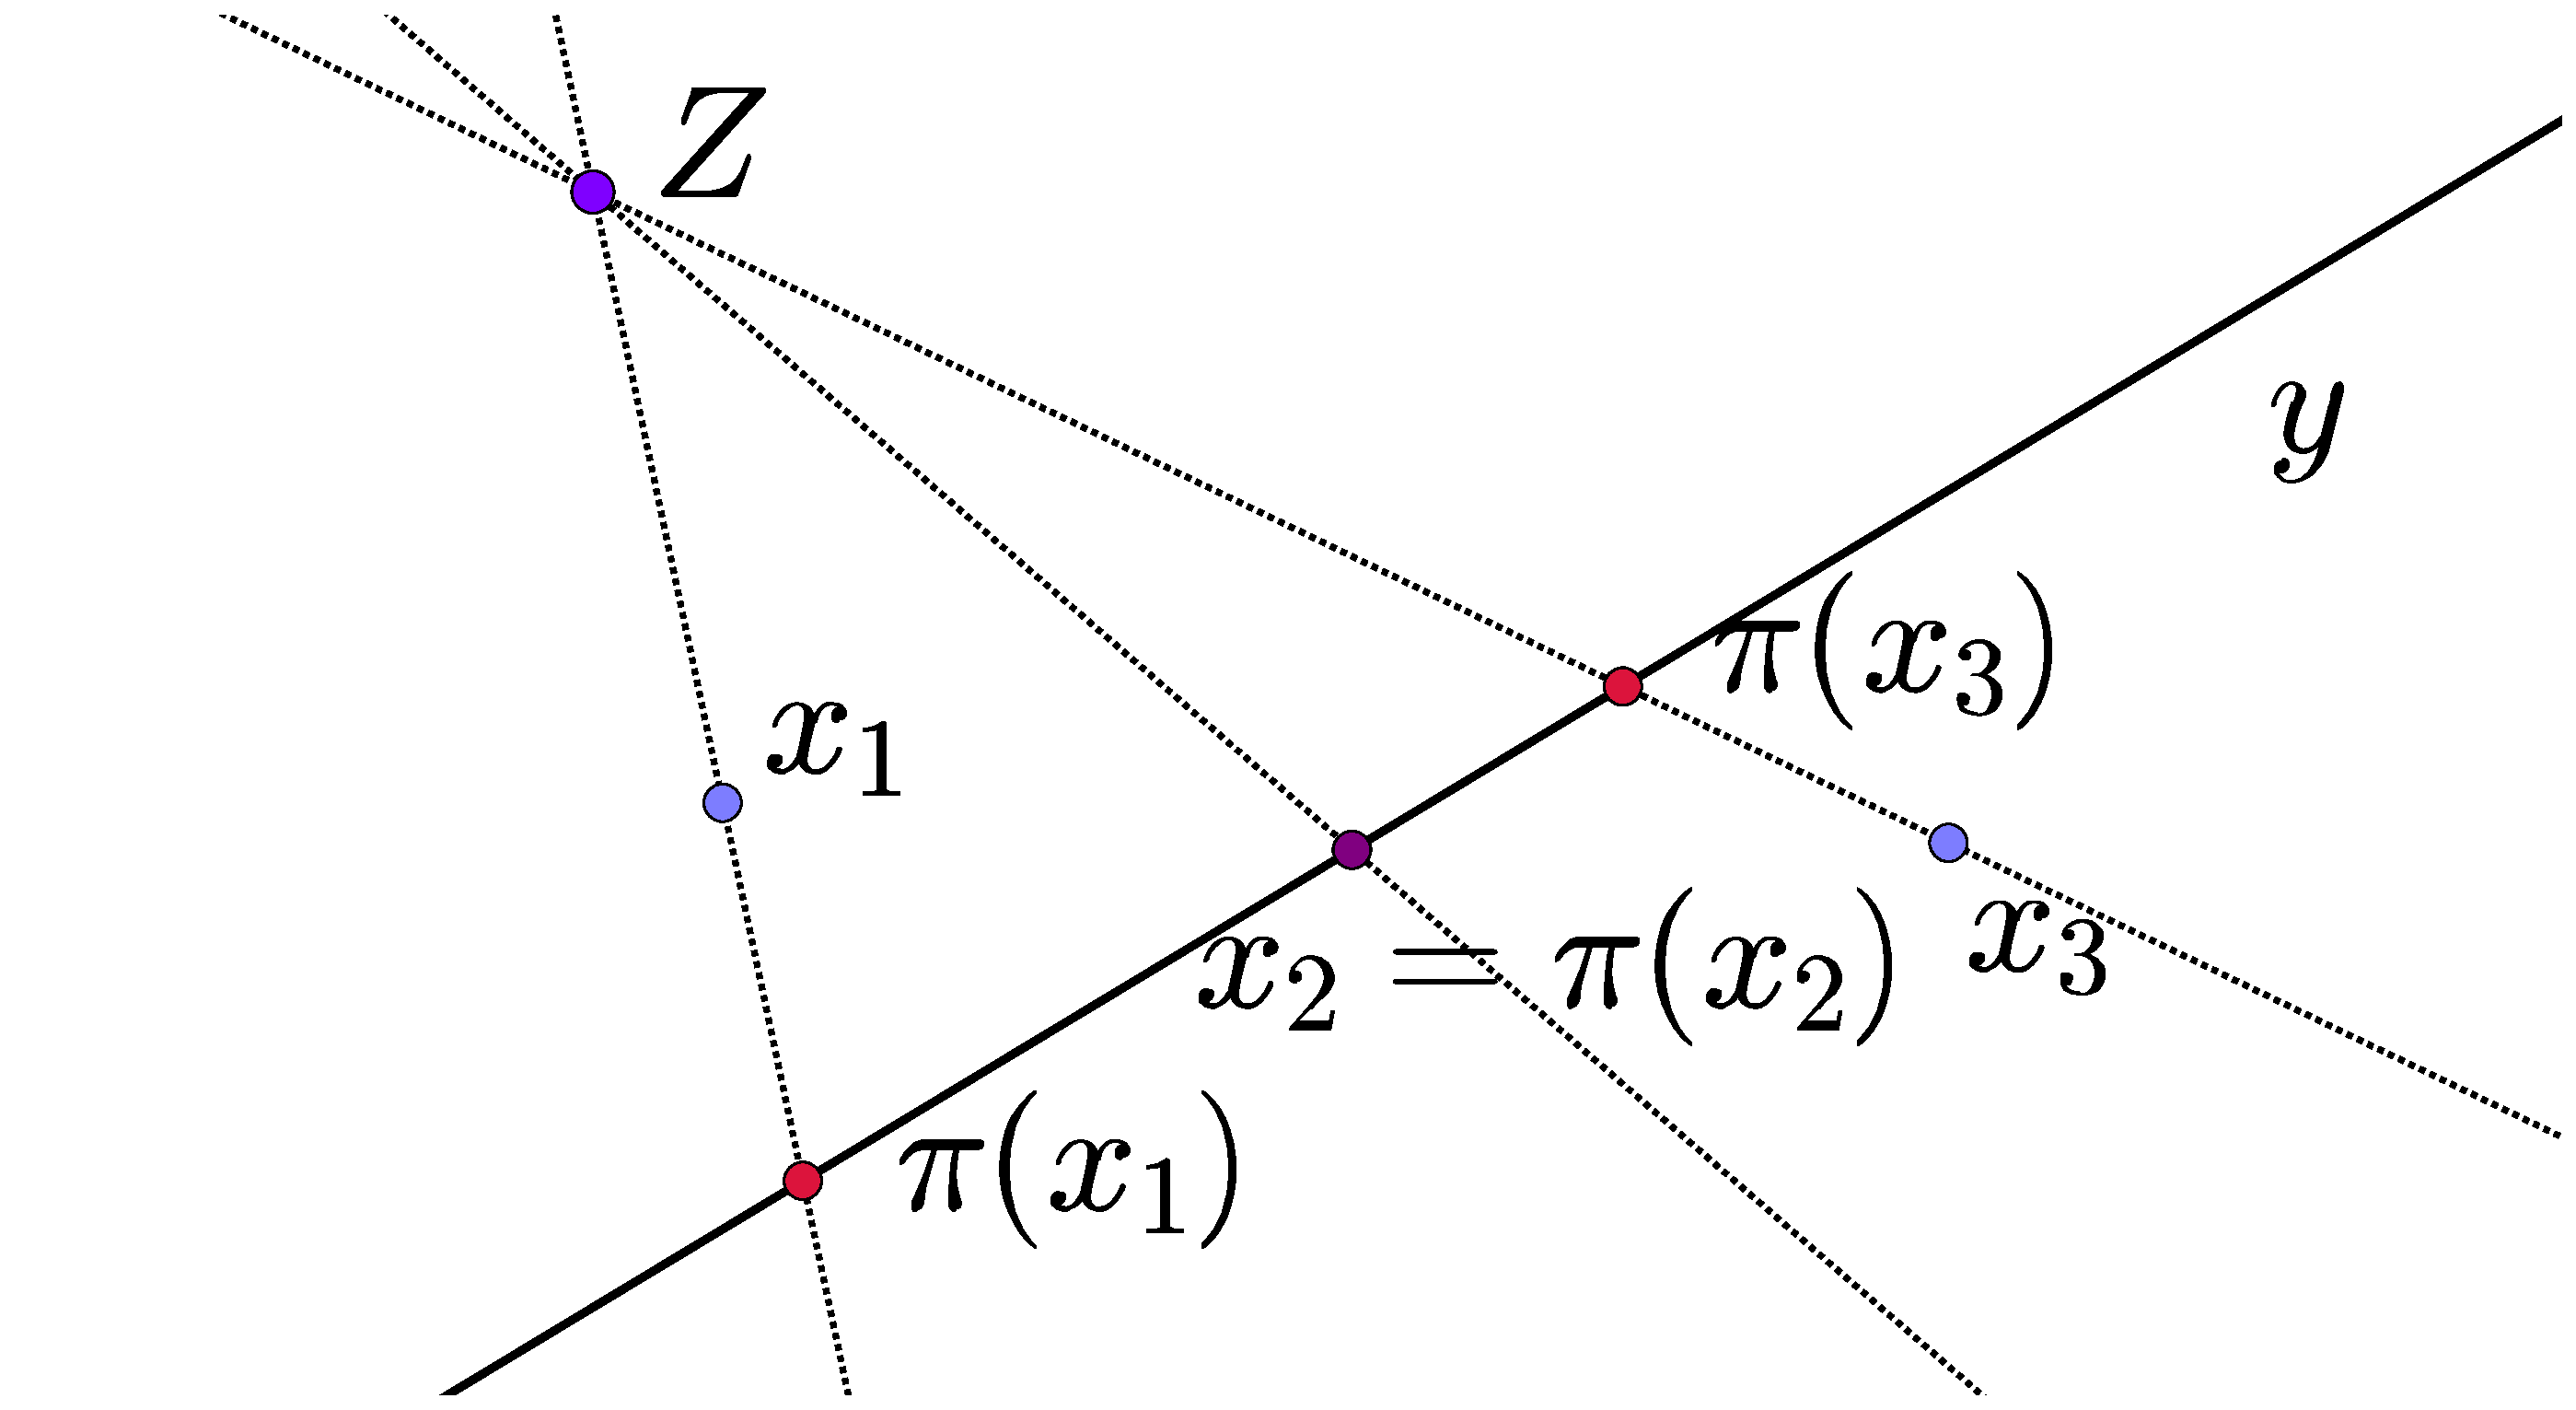
\includegraphics[scale=.15]{Graficos/rectaPunto.eps}
		\caption{Ilustración de una Proyección Punto--Recta.}
		\label{C4_puntoRecta}
	\end{figure}
	
\end{exa}

No demostraremos que la aplicación del ejemplo \ref{C4_exa_puntoRecta} es, en efecto, una aplicación proyectiva, ya que al final de la sección daremos una demostración general para todas las proyecciones cónicas, de las que esta aplicación en concreto es un caso particular.

El ejemplo \ref{C4_exa_puntoRecta} se puede generalizar para dimensiones superiores, basta mantener que $z$ sea un punto de $\proy^n$ e $Y$ un hiperplano.
\begin{exa}[Punto sobre Hiperplano]
	\label{C4_exa_puntoHiperplano}
	En el plano proyectivo $\proy^n$ consideramos el punto $z$ y el hiperplano $Y$ tal que $z\not\in Y$. Definimos la aplicación:
	\[\begin{array}{c}
	\proy^n\setminus\{z\}\stackrel{h}{\to} Y\\
	x\mapsto h(x)=\engen{x,z}\cap Y
	\end{array}\]
\end{exa}
Otra generalización de los ejemplos anteriores es la siguiente (menos intuitiva y más dificil de ver):
\begin{exa}[Recta sobre Recta]
	En el espacio proyectivo $\proy^3$ se consideran las rectas $l$ y $l'$ tales que $l\cap l'=\emptyset$. Definimos la aplicación:
	\[\begin{array}{c}
	\proy^3\setminus l\stackrel{h}{\to}l'\\
	x\mapsto\engen{x,l}\cap l'
	\end{array}\]
	Observamos simplemente que $\engen{x,l}$ siempre se corta con $l'$ en un punto (consecuencia inmediata de la fórmula de Grassmann).
	
	IMAGEN
\end{exa}

Llegados a este punto, ha llegado la hora de definir \ti{proyección cónica} en toda su generalidad.
\begin{defi}[Proyección Cónica]
	\label{C4_def_proyeccionConica}
	Sean $X$ un espacio proyectivo y $Z$ e $Y$ dos variedades proyectivas de $X$ tales que:
	\begin{enumerate}
		\item $Z\cap Y=\emptyset$
		\item $\dim(Z)+\dim(Y)=\dim(X)-1$
	\end{enumerate}
	Definimos la aplicación:
	\[\begin{array}{c}
	X\setminus Z\stackrel{h}{\to} Y\\
	x\mapsto\engen{x,Z}\cap Y
	\end{array}\]
\end{defi}
Automáticamente se nos presentan una serie de cuestiones que trataremos de responder a continuación:
\begin{enumerate}
	\item ¿La intersección $\engen{x,Z}\cap Y$ es siempre un único punto?
	\item ¿$h$ es una aplicación proyectiva? ¿Cuál es su aplicación lineal asociada?
\end{enumerate}
Como diría Jack el Destripador, vayamos por partes:
\begin{prop}[Intersección Unipuntual]
	\label{C4_prop_interseccionUnipuntual}
	En las condiciones de la definición \ref{C4_def_proyeccionConica} la intersección $\engen{x,Z}\cap Y$ tiene dimensión nula. Es decir, es un punto proyectivo.
\end{prop}
\begin{proof}
	Usando la fórmula de Grassmann:
	\begin{equation}
		\label{C4_eq_interseccionUnipuntual1}
		\dim\engen{\engen{x,Z},Y}=\dim\engen{x,Z}+\dim\engen{Y}-\dim\engen{x,Z}\cap Y
	\end{equation}
	En primer lugar, veamos cuál es la dimensión de $\engen{x,Z}$, para lo cual usaremos, de nuevo, la fórmula de Grassmann.
	\begin{equation}
		\label{C4_eq_interseccionUnipuntual2}
		\dim\engen{x,Z}=\dim(x)+\dim(Z)+\dim(x\cap Z)
	\end{equation}
	Como $\dim(x)=0$ (por ser un punto) y la dimensión de $\dim(x\cap Z)=-1$, ya que, por definición de proyección cónica $x\not\in Z$, y por tanto $x\cap Z=\emptyset$. Sustituyendo en \eqref{C4_eq_interseccionUnipuntual2} se obtiene:
	\begin{equation}
		\label{C4_eq_interseccionUnipuntual3}
		\dim\engen{x,Z}=\dim(Z)+1
	\end{equation}
	Sustituyendo este resultado en \eqref{C4_eq_interseccionUnipuntual1} obtenemos:
	\begin{equation}
		\label{C4_eq_interseccionUnipuntual4}
		\dim\engen{\engen{x,Z},Y}=\dim(Z)+1+\dim\engen{Y}-\dim\engen{x,Z}\cap Y
	\end{equation}
	Como, por hipótesis $\dim(Z)+\dim(Y)=\dim(X)-1$, sustituyendo en \eqref{C4_eq_interseccionUnipuntual4} queda:
	\begin{equation}
		\label{C4_eq_interseccionUnipuntual5}
		\dim\engen{\engen{x,Z},Y}=\dim(X)-\dim\engen{x,Z}\cap Y
	\end{equation}
	Centrémonos ahora en el otro miembro de la igualdad. En primer lugar, es claro que:
	\[\dim\engen{\engen{x,Z},Y}=\dim\engen{x,Z,Y}\]
	Parece intuitivo pensar que $Z$ e $Y$ generan $X$. Veámoslo:
	\begin{equation}
		\label{C4_eq_interseccionUnipuntual6}
		\dim\engen{Z,Y}=\dim(Z)+\dim(Y)-\dim(Z\cap Y)
	\end{equation}
	Como, por hipótesis, $Z\cap Y$ es el vacío, y, además, la suma de las dimensiones de $Z$ e $Y$ dan la dimensión de $X$ menos $1$, nos queda que, efectivamente:
	\begin{equation}
		\label{C4_eq_interseccionUnipuntual7}
		\dim\engen{Z,Y}=\dim(X)
	\end{equation}
	Por ende, $\dim\engen{Z,Y,x}=\dim(X)$, y, podemos sustituir en \eqref{C4_eq_interseccionUnipuntual5}:
	\begin{equation}
		\label{C4_eq_interseccionUnipuntual8}
		\dim(X)=\dim(X)-\dim\engen{x,Z}\cap Y
	\end{equation}
	Despejando, el resultado se sigue inmediatamente.
\end{proof}
La proposición \ref{C4_prop_interseccionUnipuntual} prueba que $h$ está bien definida como aplicación.

Una pequeña observación antes de probar que las proyecciones cónicas son, efectivamente, aplicaciones proyectivas, es que los espacios lineales asociados a $Z$ y a $Y$ son complementarios.
\begin{obs}[Espacios Lineales Complementarios]
	\label{C4_obs_espaciosComplementarios}
	Como la intersección de las variades proyectivas $Z$ e $Y$ es el vacío, esta intersección tiene dimensión $-1$. Por ende, el espacio lineal asociado a esta intersección es el nulo. Es decir:
	\[Z\cap Y=\emptyset\sii\widehat{Z}\cap\widehat{Y}=\zset\]
	Además, la suma de las dimensiones de $Z$ e $Y$ es la dimensión de $X$ menos $1$. Usando esto:
	\begin{multline*}
		\dim(Y)+\dim(Z)=\dim(X)-1\sii\\
		\sii \dim(\widehat{Y})-1+\dim(\widehat{Z})-1=\dim(\widehat{X})-1-1\sii\\
		\sii \dim(\widehat{Y})+\dim(\widehat{Z})-2=\dim(\widehat{X})-2\sii\\
		\sii \dim(\widehat{Y})+\dim(\widehat{Z})=\dim(\widehat{X})
	\end{multline*}
	En su conjunto, esto quiere decir que se tiene la siguiente descomposición en suma directa del espacio lineal:
	\[\widehat{X}=\widehat{Y}\oplus\widehat{Z}\]
\end{obs}
Probemos ahora que las proyecciones cónicas son aplicaciones proyectivas. Y que, de hecho, son las aplicaciones proyectivas asociadas a \ti{proyecciones vectoriales}. (De ahí surge el nombre de ``proyección'').
\begin{prop}[Proyección Vectorial]
	\label{C4_prop_proyeccionVectorial}
	La aplicación $h$ tiene a la siguiente aplicación lineal (proyección vectorial de $\widehat{X}$ sobre $\widehat{Y}$) como asociada:
	\[\begin{array}{c}
	\widehat{X}=\widehat{Z}\oplus\widehat{Y}\stackrel{\widehat{h}}{\to}\widehat{Y}\\
	u=v+w\mapsto w
	\end{array}\]
	Siendo $v\in \widehat{Z}$ y $w\in \widehat{Y}$, es decir, la descomposición de $x$ en suma de vectores de $\widehat{Z}$ e $\widehat{Y}$.
\end{prop}
\begin{proof}
	Comprobar que $\widehat{h}$ es una aplicación lineal con núcleo $\widehat{Z}$ es inmediato y se deja al lector. Hecho esto, suponiendo que $x=\class{u}$, basta ver que $h(x)=\class{\widehat{h}(u)}$ para cualquier $x\in X$.
	
	\[\class{\widehat{h}(u)}=\class{\widehat{h}(v+w)}=\class{w}\]
	
	Veamos que $\class{w}\in \engen{x,Z}\cap Y$, demostrando así lo que queríamos.
	
	En primer lugar, sabemos que $w$ no es el vector nulo, ya que si lo fuera, el rayo $x$ estaría en el centro. Dicho esto, como $Y=\proy(\widehat{Y})$, y como $w\in\widehat{Y}$, entonces $\class{w}\in Y$.
	
	Para demostrar que $\class{w}\in\engen{x,Z}$ basta con darse cuenta de que $\engen{x,Z}=\proy({\lengen{u,\widehat{Z}}})$. Como $u = v+w$ se tiene que $w=u-v\in\lengen{u, \widehat{Z}}$, luego, tomando clases: \[\class{w}=\class{u-v}\in\proy(\lengen{u,\widehat{Z}})=\engen{x,Z}\]
\end{proof}
La proposición \ref*{C4_prop_proyeccionVectorial} demuestra que las proyecciones cónicas en general son aplicaciones proyectivas, dando la aplicación lineal asociada (una proyección vectorial).

Antes de finalizar la sección daremos una explicación del por qué del apellido ``cónicas'' de estas aplicaciones. Además, daremos dos ejemplos detallados para que el lector se familiarice con el tratamiento de estas aplicaciones, y que, además, constituye un gran repaso de capítulos anteriores. Por último propondremos un ejercicio al lector.

\begin{obs}[Cónicas]
	\label{C4_obs_conicas}
	Este apellido es debido a que, en el caso particular presentado en el ejemplo \ref{C4_exa_puntoHiperplano}, si tomamos la imagen de una circunferencia por la proyección cónica obtenemos una curva cónica. Esta curva es la formada por la intersección entre el hiperplano $Y$ la familia de rectas que pasan por $z$ y un punto de la circunferencia.
\end{obs}

El siguiente ejemplo ilustra la importancia de asegurarse de que cumplimos con todos los requisitos a la hora de difinir una proyección cónica.
\begin{exa}[Proyección Punto -- Plano Degenerada]
	Dado el punto $z=(1:0:-1:1)$ y el plano $\pi:2x-y+z-t=0$, se pide hallar la imagen de un punto genérico $p=(x:y:z:t)$ por la proyección cónica con centro $z$ sobre $\pi$.
	
	Por definición tenemos que $h(p)=zp\cap\pi$. Dicho de otra forma, nuestro trabajo se reduce a calcular la intersección de una recta y un plano. Como tenemos el plano $\pi$ expresado en forma de su ecuación implícita, tratemos de hallar las ecuaciones paramétricas de $zp$. Estas son, en su versión no homogénea:
	\[zp:\class{(x+\theta:y:z-\theta:t+\theta)}\]
	Así pues ahora solo basta con sustituir en la ecuación implítita de $\pi$ y despejar $\theta$. Sin embargo:
	\[2(x+\theta)-y+(z-\theta)-(t+\theta)=0\sii2x-y+z-t=0\]
	Como vemos, $\theta$ se ha esfumado en el proceso. ¿Como debemos interpretar este resultado? Bueno, quizá ayude imaginarse que $p$ es un punto concreto, es decir, que las variables $x,y,z,t$ de la anterior ecuación son ``numeracos''.
	
	Hecho esto, nos quedará un número igualado a $0$. Si esta igualdad es falsa uno podría pensar que la recta no corta al plano nunca (ya que no lo hace para ningún valor de $\theta$), pero esto sabemos que no es así, ya que una recta y un hiperplano siempre se cortan. Es en este momento cuando hay que recordar que hay ocasiones en las que $\theta$ no está definido, en concreto, ningún valor de $\theta$ nos define el punto $z$. Por ende, este es el punto de corte.
	
	En otro caso, nos puede quedar la igualdad trivial, que no quiere decir otra cosa que que la recta $zp$ está contenida en el plano $\pi$. Por ende, en este caso, la imagen de $p\in\pi$ no está bien definida, ya que es toda una recta.
\end{exa}
\begin{exerc}[Clasificación de Proyecciones Cónicas]
	Enumere las proyecciones cónicas de $\proy^4$, clasificándolas en función de las subvariedades $Z$ e $Y$ que las caracterizan.
\end{exerc}
\section{Homografías}
En esta sección introduciremos unas aplicaciones proyectivas bastante notables, las llamadas ``homografías'', que se estudiaran con enorme profundidad en capítulos posteriores.
\begin{defi}[Homografía]
	\label{C4_def_homografia}
	Una aplicación proyectiva $h$ se dice \ti{homografía} si es inyectiva, es decir, si su centro es el vacío.
\end{defi}
Antes de empezar a desgranar las propiedades de estas aplicaciones, pongamos un ejemplo notable que nos permitirá construir homografías en el plano proyectivo.
\begin{exa}[Fábrica de Homografías]
	\label{C4_exa_fabricaHomografias}
	Sean $r$ y $r'$ dos rectas distintas de $\proy^2$. Asimismo un punto proyectivo $c\in\proy^2\setminus\{r\cup r'\}$.
	
	Definimos la aplicación: \[\begin{array}{c}
	\pi_c:r\to r'\\
	p\mapsto \engen{c,p}\cap r'
	\end{array}\]
	
	Esta aplicación es una homografía, de hecho, es una restricción de la aplicación definida en el ejemplo \ref{C4_exa_puntoRecta}. En definitiva, dado un punto y dos rectas, tenemos una homografía.
	
	IMAGEN
\end{exa}

Una propiedad importante de las homografías es que pueden transformarse de forma natural a en aplicaciones biyectivas.
\begin{obs}[Biyectividad de las Homografías]
	Al ser las homografías aplicaciones inyectivas, si la dimensión del espacio de partida y de llegada coinciden, la aplicación en cuestión es biyectiva. Este hecho se debe a la fórmula de las dimensiones para aplicaciones lineales.
	
	En caso de que esto no ocurra, siempre podemos tomar como espacio de llegada la imagen de la aplicación en sí, que será un espacio proyectivo de la misma dimensión que el de partida.
\end{obs}

\subsection{Homografías y Teoría de Grupos}
Algo objetivamente bonito de las homografías es que se relacionan muy fácilmente con la teoría de grupos. Así es como surge el concepto de ``grupo proyectivo''.
\begin{defi}[Grupo Proyectivo]
	Sea $X$ un espacio proyectivo. Se llama \ti{grupo proyectivo} de $X$ al conjunto formado por todas las homografías de $X$ en sí mismo con la operación de composición usual. A este grupo se le suele denotar $\mathbf{GP}(X)$.
\end{defi}
La comprobación de que, efectivamente, el conjunto de las homografías de un subespacio en sí mismo tiene estructura de grupo es un sencillo ejercicio que se deja al lector.

Recordamos brevemente que denominábamos \ti{grupo lineal} de un espacio vectorial $\widehat{X}$ al conjunto de sus automorfismos (isomorfismos de él en sí mismo) con la composición usual. A este grupo lo denotábamos $\mathbf{GL}(\widehat{X})$.

Parece natural pensar que existe cierta relación entre los grupos lineal y proyectivo. Así es, gracias a todas las propiedades demostradas a lo largo del capítulo, podemos definir el siguiente homomorfismo sobreyectivo de grupos (compruébese).
\[\begin{array}{c}
	\mathbf{GL}(\widehat{X})\to\mathbf{GP}(X)\\
	\widehat{h}\mapsto h
\end{array}\]
A cualquiera que haya estudiado teoría de grupos esto le pide a gritos que calculemos el kernel del homomorfismo y apliquemos el llamado \ti{Primer Teorema de Isomorfía}. Hagámoslo.

El elemento unidad del grupo proyectivo es la aplicación identidad, que lleva cada punto a sí mismo, como es claro que la aplicación lineal identidad es la asociada a esta aplicación proyectiva, también lo serán todos sus múltiplos (y solo esos) (teorema \ref{C4_teo_lemaCorrespondencia}), con lo que queda calculado el kernel del homomorfismo, que es, por supuesto, un subgrupo normal de $\mathbf{GL}(\widehat{X})$.

A los múltiplos de la aplicación lineal identidad usualmente se les denomina \ti{homotecias lineales}. Denominaremos $H$ al conjunto de las homotecias lineales.

Aplicando el primer teorema de isomorfía tenemos que:
\[\mathbf{GP}(X)\cong\frac{\mathbf{GL}(\widehat{X})}{H}\]

Sin embargo, podemos ir aún más allá. Consideremos el siguiente homomorfismo inyectivo:
\[\begin{array}{c}
\K^*\to\mathbf{GL}(\widehat{X})\\
\lambda\mapsto\lambda\mathrm{id}
\end{array}\]

Luego por el primer teorema de isomorfía se tiene que $\K^*$ es isomorfo a $H$ con lo que concluimos:
\begin{equation}\mathbf{GP}(X)\cong\frac{\mathbf{GL}(\widehat{X})}{\K^*}\end{equation}
\section{Aplicaciones Proyectivas y Matrices}
Uno de los resultados más notables y relevantes del álgebra lineal es que una aplicación lineal queda totalmente determinada por la imagen de los vectores la base del espacio de partida. Tratemos de traducir esto al contexto de las aplicaciones proyectivas.


\subsection{Recordatorio de Álgebra Lineal} 

Recordamos que, dado un vector $u\in E$ y un homomorfismo $h:E\to E'$, fijadas sendas bases $\mc{B}$ y $\mc{B}'$ de $E$ y $E'$ se tiene:
\begin{equation}
	\label{C4_eq_formulaLineales}
	h(u)\equiv Y=M_{\mc{B}\mc{B}'}(h)X
\end{equation}
En este contexto, $X$ representa una matriz columna cuyos coeficientes se corresponden con las coordenadas del vector $u$ respecto de $\mc{B}$. Análogamente, $Y$ es una matriz columna cuyos coeficientes son las coordenadas de $h(u)$ respecto de $\mc{B}'$. Por su parte, $M_{\mc{B}\mc{B}'}(h)$ es la llamada \ti{matriz asociada a $h$} respecto de $\mc{B}$ y $\mc{B}'$. Las columnas de la matriz $M_{\mc{B}\mc{B}'}(h)$ se corresponden con las coordenadas en la base $\mc{B}'$ de la imagen de los vectores de la base $\mc{B}$. 

Asimismo conviene recordar qué relación había entre $M_{\mc{B}\mc{B}'}(h)$ y $M_{\overline{\mc{B}}\overline{\mc{B}'}}(h)$. Esta relación era:
\begin{equation}
	M_{\overline{\mc{B}}\overline{\mc{B}'}}(h)=Q^{-1}M_{\mc{B}\mc{B}'}(h)P
\end{equation}
Donde $P^{-1}$ y $Q^{-1}$ son, respectivamente, las matrices de cambio de base de $\mc{B}$ a $\overline{\mc{B}}$ y de $\mc{B}'$ a $\overline{\mc{B}'}$. (Ver apéndice \ref{A1_cambioBase}).
\subsection{Matriz Asociada a una Aplicación Proyectiva}
Sean dos espacios proyectivos $X$ e $Y$. Consideremos las referencias proyectivas $\mf{R}$ y $\mf{R}'$ asociadas a $X$ e $Y$ respectivamente. Definamos una aplicación proyectiva $h:X\setminus \mc{Z}\to Y$ arbitraria.

Nuestro objetivo es, dadas las coordenadas homogéneas de cierto rayo $\class{w}\in X$ respecto de $\mf{R}$, obtener las coordenadas homogéneas $h(\class{w})\in Y$ respecto de $\mf{R}'$.

Denotando por $W$ a la matriz columna cuyos coeficientes son las coordenadas homogéneas de $w$ respecto de $\mf{R}$ (únicas salvo múltiplos). Se cumple que:
\begin{equation}
	h(\class{w})=\class{\widehat{h}(w)}\equiv\class{M_{\mc{B}\mc{B}'}(\widehat{h})W}
\end{equation}
Nótese que hemos cometido un abuso de notación ya que $M_{\mc{B}\mc{B}'}(\widehat{h})W$ es una matriz columna, sin embargo la consideramos como un vector para poder tomar el rayo engendrado por él.

Que no cunda la euforia, todavía tenemos un problema por subsanar, ya que al ser las bases asociadas a $\mf{R}$ y $\mf{R}'$ únicas salvo múltiplos nadie me impide coger la base $\lambda\mc{B}$ (para cierto escalar $\lambda$ no nulo) en lugar de la base $\mc{B}$.

Sin embargo, las matrices de cambio entre bases asociadas (y sus inversas) son múltiplos de la identidad (por ser las unas múltiplos de las otras). Esta propiedad trae a colación un viejo resultado acerca de matrices que reza que al multiplicar una matriz (ya sea por la izquierda o por la derecha) por $\lambda I_n$ es equivalente a multiplicar la matriz por $\lambda$. Así pues tenemos que:
\begin{equation}
	\class{M_{\lambda \mc{B}\mu\mc{B}'}(\widehat{h})W}=\class{M_{\mc{B}\mc{B}'}(\widehat{h})\lambda\mu W}=\class{M_{\mc{B}\mc{B}'}(\widehat{h})W}=:h(\class{w})
\end{equation}
Pongamos algunos ejemplos para asentar todo esto.
\begin{exa}[Transformaciones de Möbius]
	\label{C4_exa_mobius}
	Sea $h:\proy^1\to\proy^1$ una aplicación proyectiva. Consideramos la referencia $\mf{R}:=\{\class{u},\class{v};e\}$ cuya base asociada es $\mc{B}=\{u,v\}$, tanto en el espacio de llegada como en el de salida. Sabemos además que $\widehat{h}(u)=au+bv$ y que $\widehat{h}(v)=cu+dv$.
	
	Sea un punto $x=(x_0:x_1)_{\mf{R}}$, por lo que acabamos de ver, su imagen por $h$ es:
	\[h(x)=\class{\rho(y_0,y_1)^t}=\class{\begin{pmatrix}
	a & c\\
	b & d
	\end{pmatrix}\begin{pmatrix}
	x_0\\
	x_1
	\end{pmatrix}}\]
	Usualmente lo escribiremos de forma ecuacional:
	\[\begin{array}{l}
	\rho y_0 = ax_0+cx_1\\
	\rho y_1 = bx_0+dx_1
	\end{array}\]
	Podríamos quedarnos ahí, sin embargo seguiremos el proceso de ``deshomogeneización'' habitual, que nos será de gran utilidad en el futuro.
	
	Dividiendo sendas ecuaciones queda:
	\[\frac{y_0}{y_1}=\frac{ax_0+cx_1}{bx_0+dx_1}\]
	Si además dividimos el término de la derecha por $x_1$ tenemos:
	\[\frac{y_0}{y_1}=\frac{a\frac{x_0}{x_1}+c}{b\frac{x_0}{x_1}+d}\]
	Denotando $\theta':=\frac{y_0}{y_1}$ y $\theta:=\frac{x_0}{x_1}$ nos queda:
	\[\theta'=\frac{a\theta+c}{b\theta+d}\]
	
	Antes de que se nos lapide por blasfemos, nótese que, como es evidente, hay ideterminaciones. En efecto cuando la segunda componente homogénea de nuestro punto inicial es nula el valor $\theta$ no está definido. Cuando esto pasa, el valor $\theta'$ es:
	\[\theta'=\frac{ax_0}{bx_0}=\frac{a}{b}\]
	Lo cual siempre está definido (salvo que $b$ sea nulo). Es por esto que a veces se toma el siguiente convenio notacional, que hace realidad el sueño de todo chaval. Asignamos a $\theta$ el símbolo $\infty$ y operamos de la siguiente manera tan intuitiva (y peligrosa):
	
	\[\theta'=\frac{a\infty+c}{b\infty+d}=\frac{a\cancel{\infty}}{b\cancel{\infty}}=\frac{a}{b}\]
	Aunque puede seguirse este convenio (y en ocasiones lo haremos), ante la duda, se recomienda pasar todo al terreno estable de las coordenadas homogéneas.
	
	Para no perder el contexto, nótese que ahora nuestro punto inicial $x$ queda totalmente determinado por $\theta$ (admitiendo que pueda tomar como valor el símbolo $\infty$ cuando la segunda coordenada homogénea sea $0$, ya que al fin y al cabo esto sólo pasa para un único rayo).
	
	Asimismo, $h(x)$ queda totalmente determinado por el valor $\theta'$, asumiendo a su vez que puede tomar como valor $\infty$ cuando su segunda coordenada homogénea se anule. Usualmente cometeremos un abuso de notación escribiendo $h(\theta)=\theta'$.
	
	Estas transformaciones son de enorme utilidad en el análisis complejo, es por ello que tienen nombre propio, \ti{transformaciones de Möbius}.
\end{exa}
En este ejemplo se generalizamos la idea del anterior para una proyección cónica.
\begin{exa}[Proyección Punto -- Plano]
	Dado el punto $z=(1:0:-1:2)$ y el plano $\pi:2x-y+z-t=0$, se pide hallar la imagen de un punto genérico $p=(x:y:z:t)$ por la proyección cónica con centro $z$ sobre $\pi$.
	
	Por definición, $h(p)=zp\cap\pi$. Hallemos las ecuaciones paramétricas de la recta $zp$ para sustituir en la ecuación paramétrica de $\pi$ y así hallar la intersección.
	\[zp:(x+\theta:y:z+\theta:t+\theta)\]
	Sustituyendo en la ecuación implícita de $\pi$ y despejando $\theta$ obtenemos:
	\[\theta=-\frac{1}{2}(2x-y+z-t)\]
	De este modo, la imagen por $h$ de un punto $p$ arbitrario es:
	\[h(p)=(y-z+t:2y:-2x+y+z+t:-2x+y-z+3t)\]
	Algunos consejos para comprobar si, en efecto, hemos echado bien las cuentas son:
	\begin{itemize}
		\item Comprobar que el punto $z$ no debe tener imagen definida, es decir, nos debe dar el punto $(0:0:0:0)$.
		\item Comprobar que los puntos del plano $\pi$ quedan invariantes por $h$.
	\end{itemize}
	Una vez hecho esto podemos hallar la matriz asociada a la aplicación lineal subyacente. Para ello basta hallar las imaǵenenes de los rayos asociados a la base canónica de $\R^4$. Nos queda:
	\[\begin{pmatrix}
	0 & 1 & -1 & 1\\
	0 & 0 & 2 & 0\\
	-2 & 1 & 1 & 1\\
	-2 & 1 & -1 & 3
	\end{pmatrix}\]
	Esta matriz tiene rango $3$ ya que la aplicación proyectiva tiene un punto por centro.
	
	Expresemos esto de forma ecuacional, simplemente porque podemos:
	\[
	\begin{array}{l}
		\rho x'= y-z+t\\
		\rho y'= 2y\\
		\rho z'= -2x+y+z+t\\
		\rho t'= -2x+y-z+3t
	\end{array}
	\]
	Tal y como hicimos en el ejemplo anterior (aquí lo hacemos con mucho menos detalle), podemos realizar el proceso de deshomogeneización habitual dividiendo todo por la última ecuación y, tras esto, dividiendo los miembros de la derecha por $t$. Si lo hacemos nos queda:
	\[
	\begin{array}{ccc}
	X'=\frac{Y-Z+1}{-2X+Y-Z+3} &
	Y'=\frac{2Y}{-2X+Y+Z+3} &
	Z'=\frac{-2X+Y+Z+1}{-2X+Y-Z+3}
	\end{array}
	\]
	que se pueden considerar las ecuaciones de la proyección en coordenadas no homogéneas. Observemos que hemos introducido las notaciones:
	\[\begin{array}{ccc}
	X'=\frac{x}{t} & Y'=\frac{y}{t} & Z'=\frac{z}{t}
	\end{array}\]
	Es claro que en todo este proceso quedan por definir un montón de singularidades, en concreto, queda indefinido todo el plano $\pi':-2x+y-z+3t=0$, que puede interpretarse como el plano paralelo a $\pi$ que pasa por $z$. En efecto, este plano lo conforman puntos cuya imagen a través de la proyección, como siempre, viene definida por $h(p)=zp\cap \pi$. Dado que $h(p)=\infty$ para todo punto $p\in\pi'$, la intersección es el infinito, por lo que $\pi'$ debe ser paralelo a $\pi$, y no puede ser otro que el plano paralelo a $\pi$ que pasa por $z$.
\end{exa}
Antes de finalizar el capítulo, hagamos un pequeño inciso. Cuando trabajemos con aplicaciones de un espacio en sí mismo conviene fijar la misma referencia $\mf{R}$ para ambos espacios. Veamos un ejemplo de por qué esto es conveniente.
\begin{exa}[Identidad]
	Sea $h:\proy^1\to\proy^1$ una aplicación proyectiva. Fijada la referencia proyectiva $\mf{R}:=\{\class{u},\class{v};e\}$ del espacio de partida, supongamos que $h$ es tal que podemos fijar la referencia protectiva $\mf{R}':=\{h(\class{u}),h(\class{v});h(e)\}$ del espacio de llegada.
	
	Se tiene entonces que la matriz asociada a la aplicación lineal asociada es la identidad. Este hecho perturba bastante a la hora de trabajar, por lo que debemos evitarlo, tomando la misma referencia.
\end{exa}